\documentclass[conference]{IEEEtran}
\usepackage{amsmath,amsfonts,amssymb}
\usepackage{graphicx}
\usepackage{cite}
\usepackage{url}
\usepackage{booktabs} % For better table lines
\usepackage{multirow} % For multirow cells in tables
\usepackage{lettrine} % For drop cap
\usepackage{balance} % To balance columns on the last page
\usepackage{tikz}
\usetikzlibrary{shapes.geometric, arrows.meta, positioning}
\usepackage{url}
\tikzstyle{box} = [rectangle, minimum width=5.5cm, minimum height=1.2cm, text centered, draw=black]
\tikzstyle{arrow} = [thick,->,>=stealth]

\begin{document}

\title{Hybrid Deep Learning for Robust Deepfake Video Detection with Enhanced Generalization and Fairness}



\author{
\IEEEauthorblockN{Paras Garg\IEEEauthorrefmark{1}, Mayank Dave\IEEEauthorrefmark{2}}\\ 
\IEEEauthorblockA{
Department of Computer Engineering\\
National Institute of Technology, Kurukshetra\\ Haryana-136119, India\\
Email: \IEEEauthorrefmark{1}324103210@nitkkr.ac.in, \IEEEauthorrefmark{2}mdave@nitkkr.ac.in
}
}


\maketitle

\begin{abstract}
The fast growth in generative artificial intelligence is causing serious problems in trusting digital media public confidence issues, and instability in society. As malicious applications involve disinformation, financial fraud, and privacy violations, it is  necessary to create secure ways of finding them. This paper introduced a hybrid deep learning architecture that finds whether a video is authentic or manipulated by detecting inconsistencies between frames of a video. The proposed architecture compromises of mainly three models, i.e. ResNet50, Bi-GRU, Multi-Head Attention. Each model has its own unique importance in detecting inconsistencies. Convolutional Neural Networks like ResNet50 are an important part of the architecture, they help to spatially analyze the video, Bi-GRUs are included for temporal analysis, and Multi-Head Attention helps to focus on certain parts of the video and how they are changing across frames. Training is performed on a strategically put together dataset made up of FaceForensics++, Celeb-DF, and the Deepfake Detection Challenge (DFDC) to enhance generalization and to minimize biases in the datasets. Extensive tests and ablation studies show that this design works well to detect similar forgery signs and produces better results than current leading methods, specifically in 'real world' and mixed-group content. It is clear from the findings that having several ways to check the truth of videos and using diverse training resources are useful for countering threats.
\end{abstract}

\begin{IEEEkeywords}
Deepfake Detection, Hybrid Deep Learning, Convolutional Neural Networks, Recurrent Neural Networks, Attention Mechanism, Generalization, and Fairness.
\end{IEEEkeywords}

\section{Introduction}
Since Artificial Intelligence and Machine Learning have advanced in recent years, creating deepfakes has become simple and increasingly accurate. Advanced deep learning helps to edit images and videos so that viewers cannot tell if the scene is real or not. Generative Adversarial Networks (GANs) and autoencoders have helped advance the technology used to produce synthetic media. Diffusion models allow modern artists to create images and videos that are so lifelike they seem like photographs \cite{kaur2024deepfake}. Despite having good applications, the rise in deep-fake technology has made it available to many people who use it for evil. Since deepfakes are always improving, it becomes tougher to detect them, so detection tools must also improve. 

Generative AI models, especially GANs, VAEs, and diffusion models, have made synthetic media look much more real and lifelike. Initially, GANs put out artifacts like flickering, and VAEs might create overly smooth outcomes, but diffusion models are now able to create images and videos that appear as if they were taken with a camera. As forgery methods continue to develop, it has sparked competition between inaccurate detectors and ever-improving deepfake generators.



Deepfake technology has the potential to help, but the fact that it is now accessible to more people has allowed fraudsters to use it. Generative advances lead to more advanced manipulations which ensure that detection tools have to keep developing. Many deepfake detection techniques are vulnerable because they do not work when facing examples they were not trained on or in situations we can find in real life \cite{dissanayake2025review}. Academic benchmarks tend to report high accuracy, but their performance may drop by 50\% or more in AUC when compared to modern "in-the-wild" deepfakes. This large difference between the results for known and unknown deepfakes clearly shows that approaches are needed to detect deepfakes from many different sources.


The project seeks to solve these difficulties by developing a hybrid deep learning architecture that can distinguish between real and deepfake videos. The objectives are as follows:
\begin{itemize}
   \item  Set up and use a combination of CNNs, RNNs and attention mechanisms in a single deep learning architecture for reliable deepfake detection.
   \item   To learn and measure the performance of model in a grouped dataset from a variety of deepfake datasets to increase its general usefulness and strength.
   \item   Analyze the model to see how accurate it, is and how well it handles methods of forgery it has not seen.
\end{itemize}
The focus of this research is video-based deepfake detection, primarily by analyzing visual features and temporal inconsistencies within video sequences using publicly available deepfake datasets.

\section{Related Work}
Because creating synthetic media is now quick and easy, deepfake detection is now a very important area of research. Knowing how deepfake content is created and noticing the boundaries of current detection techniques is important for effective protection.

\subsection{Deepfake Generation Techniques}
Deepfakes have become possible due to new developments in generative AI models.
\begin{itemize}
\item \textbf{Generative Adversarial Networks (GANs) :} GAN use a competitive setup between a generator and a discriminator to produce real-looking pictures, but frequently include obvious signs like unmatched lip movements or a flickering speed.
\item \textbf{Autoencoders / Variational Autoencoders (VAEs) :} Compress and rebuild data that make face swapping possible. The results achieved in earliest times appeared sometimes too smooth and fake.
\item \textbf{Diffusion Models:} Serve as the most advanced technique in creating realistic images and videos, by beginning with noise and ending up with realistic shots, though some noise and time errors may remain.
\end{itemize}
Better forgery techniques being developed regularly encourage the use of detection methods that detect a wider range of forgery signs.



\subsection{Deepfake Detection Approaches}
Various methodologies have been explored to counter evolving generation techniques.

\subsubsection{Spatial Feature-Based Methods (CNNs)}
Deepfake detection relies heavily on Convolutional Neural Networks (CNNs) in spatial features due to their strong skills in identifying differences and unique patterns in someone’s face. Rossler et al. (2019) \cite{rossler2019faceforensics} discussed the FaceForensics++ dataset and pointed out that CNNs play a good role in detecting small changes in deceptively manipulated videos. Nguyen et al. (2019) \cite{nguyen2019capsule} introduced a capsule network that addresses location errors to produce more stable object detection. Lewis et al. (2021) \cite{lewis2020deepfake} applied attention mechanisms to CNNs to concentrate on the most important parts of faces, allowing for better detection results under lower image compression. Evidence from several studies proves that spatial feature extraction via CNNs is still the top approach to identify artifacts that make deepfakes unique. But, CNN-based systems generally perform on a single shot and may not detect conflicts between shots. These models have trouble with new kinds of fraud and when their data is similar, they can sometimes be very strict. 

\subsubsection{Temporal Feature-Based Methods (RNNs, LSTMs, GRUs)}
RNNs, LSTM and GRUs in temporal analysis search for motion artifacts and inconsistencies in videos that are usually unnoticed by methods that only consider spatial aspects. The MesoNet was proposed by Afchar et al. (2018) \cite{afchar2018mesonet} which brings together CNNs and temporal cues to detect deepfake videos accurately. LSTM networks were employed by Guera et al. (2018) \cite{guera2018deepfake} used sequential facial frames to improve detection performance by including them in the model.

\subsubsection{Hybrid and Multi-Modal Approaches}
Integrating spatial, temporal and audio information using hybrid approaches has become effective in finding deepfakes. Zhou et al. (2019) \cite{zhou2017two}.created a two-network structure with CNN for feature extraction in fixed parts of the body and RNN for learning the sequence of movement, obtaining better results through a joint analysis of frame changes and motion clues. Building on the concept, Parikh et al. (2023) \cite{parikh2023audio} used deep neural networks and examined audio features, showing that integrating across visual and audio inputs is helpful for identifying harmful changes in both streams. Li et al. (2021 \cite{huang2024spatiotemporal}) proposed a hybrid framework that combines CNN spatial features with LSTM for handling time-based data, allowing the system to pick out key locations and timeframes to spot small changes in compressed videos.





\subsection{Critical Challenges in Deepfake Detection}
Deepfake detection faces several critical challenges hindering real-world applicability.

\subsubsection{Generalization to Unseen Forgeries and Domain Shift}
A big issue is that most deepfake detectors do not work well against deepfakes used outside of experiments and new types of deepfake methods. Many performance measures used in academics are old which results in a dramatic fall in performance on contemporary “actual use” data, with AUC values dropping significantly for video models. Detectors may become biased because they respond to issues unrelated to forgery \cite{fu2025unbiased}.

\subsubsection{Dataset Bias and Fairness Disparities}
Learning algorithms may not detect crimes equally well for different people, like those from different races or genders, as a result of training data bias. Studies suggest \cite{mubarak2023survey} people with lighter skin tones are more accurately detected which leaves darker-skinned groups exposed to potential harm.

\subsubsection{Real-World Applicability and Evasion Techniques}
Because deepfake technology is designed to be deceitful, those who use it are always finding new ways to avoid being discovered. This type of competition constantly changes, so static and universal answers are not handy \cite{mubarak2023survey}. Because of issues like compression in real life, deepfakes are often different from synthetic datasets and can reduce how well models perform.



\section{Proposed Methodology}
This chapter details the proposed hybrid deep learning solution, outlining its architectural components, dataset aggregation strategy, and preprocessing steps. The design rationale for each element is rooted in addressing the critical challenges of generalization, robustness, and fairness identified in deepfake detection. This design is built upon existing hybrid approaches \cite{antad2024hybrid} \cite{rana2021ml}, aiming to improve the robust performance of the model in detecting deepfake videos.

\subsubsection{Selection of Benchmark Datasets}
The model is trained on a combination of three major deepfake benchmarks:
\begin{itemize}
    \item \textbf{FaceForensics++ (FF++):} This dataset consists of 1000 original video sequences \cite{roessler2019faceforensicspp}. These video sequences are manipulated using different face manipulation methods: Deepfakes, Face2Face, FaceSwap, and NeuralTextures. Sourced from YouTube, it provides a diverse set of manipulation techniques and is foundational for deepfake detection research.
    \item \textbf{Celeb-DF:} This dataset contains 590 original and 5,639 high-quality deepfake videos of celebrities \cite{li2020celebdf}. It is particularly challenging because its deepfakes are generated with improved synthesis processes designed to reduce common artifacts, making them visually more convincing and harder to detect than those in older datasets .
    \item \textbf{Deepfake Detection Challenge (DFDC) Dataset:} This is the largest publicly available face swapped video dataset which comprises over 100,000 clips that are sourced from 3,426 paid actors \cite{dolhansky2020dfdc}. It includes videos produced with various GAN-based and non-learned methods, and importantly, features diverse augmentations to simulate real-world conditions. Its sheer scale and diversity are crucial for learning robust and generalizable features.
\end{itemize}
Because there are so many different ways of creating forgeries, visual characteristics and subjects included, they are important for reducing potential bias in the data and making it work better on other deepfakes. By using both kinds of data, the model deals with a larger and fairer variety of information which helps reduce bias and improve how it performs on unseen data.



\subsubsection{Data Collection and Preprocessing Steps}
A unified protocol makes sure all files are in the same format and have the same labels. Pre-processing involves:
\begin{itemize}
    \item \textbf{Frame Extraction and Face Cropping:} Videos are split into individual frames 10, and a face detection algorithm crops face regions.
    \item \textbf{Resizing and Normalization:} Cropped frames are resized 112x112 pixels and pixel values normalized using ImageNet mean and standard deviation.
    \item \textbf{Frame Sampling Strategy:} A fixed frame sampling strategy 10 fps is employed for consistency.
\end{itemize}

\subsubsection{Enhancing Generalizability and Robustness by Using Data Augmentation}
Applying different data augmentations expands the variety in the dataset, prevents overfitting and makes the system more robust \cite{papakipos2022augly}. Common augmentations include:
\begin{itemize}
    \item \textbf{Geometric transformations:} Random horizontal flips, crops, rotations, scaling, and translations.
    \item \textbf{Color space transformations:} Adjustments to brightness, contrast, and saturation.
    \item \textbf{Adding noise or blurring:} Mimicking compression artifacts or low-quality captures.
\end{itemize}
In every part of a sequence, these augmentations are used consistently to ensure that everything happens in the same order.


\subsection{Proposed Hybrid Deep Learning Architecture}
The proposed hybrid architecture is designed to detect deepfake content by using spatial and temporal features of each frame combined with attention mechanism to focus on certain part of the image simultaneously. The system aims to combine the power of Convolutional Neural Networks (CNNs) for spatial representation, Recurrent Neural Networks (RNNs) for temporal feature extraction, and Multi-Head Attention for contextual focus.

\subsubsection{Spatial Feature Extraction with Convolutional Neural Networks (CNNs)}


The main idea is to use ResNet50 to extract detailed spatial features from every frame of the video. The reason to choose ResNet50 is its efficiency at performing image classification and solving the problem of vanishing gradients by using residual connections. Pre-training the model on the ImageNet-1K set helps with transfer learning which ensures strong basis for picking out common yet varying traits in facial images. It helps locate small changes in space like blurring that looks off, extra pixels on the picture or unusual frame coloring. Rather than using the original final classification layers, ResNet50 only keeps the convolutional layers which serve as strong encoders of features.

\subsubsection{Temporal Anomaly Detection with Recurrent Neural Networks (RNNs)}


The high-level spatial features extracted by ResNet50 are then individually processed by the Bi-GRU (Bi-GRU). Bi-GRUs do well with sequential data as they can capture the influence of earlier steps on later ones in both directions. Being able to look in both directions is key for catching inconsistencies in deepfake videos that occur gradually, like unrealistic eye movements, unusual head movements or flickering. Learning complex temporal patterns is important to catch any changes in the video flow and the Bi-GRU layer helps the model do so.


\subsubsection{Integration of Attention Mechanisms}



Multi-Head Attention is used after the Bi-GRU layer. This helps the model can focus on the most important segments of the data by looking at multiple features all at once, allowing it to perform better. Multi-Head Attention does this by applying weighting to the various part of the temporal sequence, so it can focus on minor shifts in images and combine details from different regions of the same pattern despite them being divided throughout the clip. It is necessary to notice deceptive changes that might go undetected with only spatial or sequential analysis.

\subsubsection{Classification Head Design}
The final classification head includes fully connected layers that map the fused feature representation to a binary decision (real or fake). Layer normalization is used to stabilize the learning dynamics and reduce internal covariate shift. The Gaussian Error Linear Unit (GELU) activation function is applied due to its smooth curvature and improved empirical performance compared to ReLU.

\subsection{System Workflow Overview}

\begin{figure}[!ht]
    \centering
    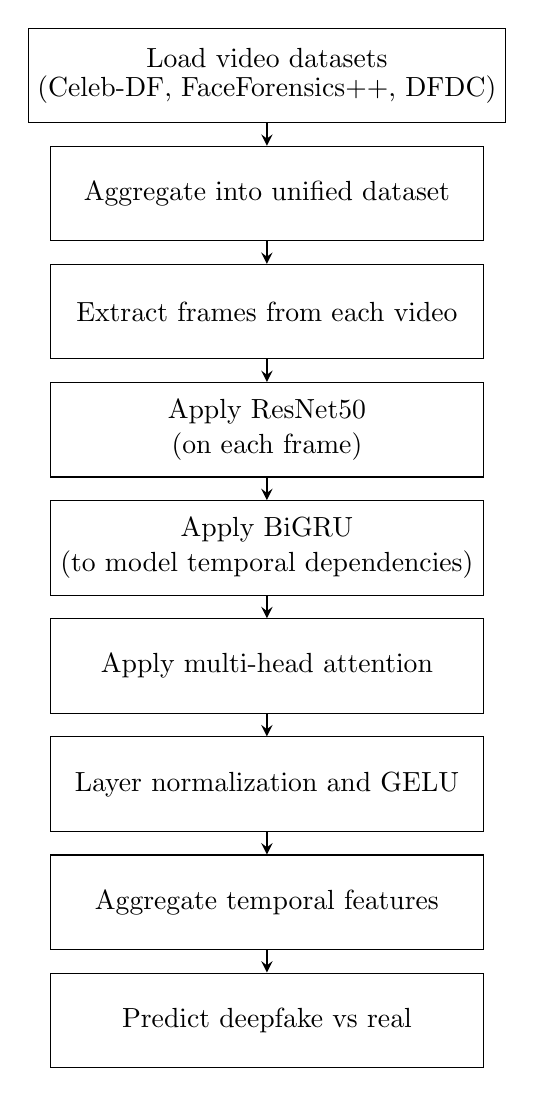
\begin{tikzpicture}[node distance=1.5cm]

    \node (load) [box] {\shortstack{Load video datasets\\(Celeb-DF, FaceForensics++, DFDC)}};
    \node (aggregate) [box, below of=load] {Aggregate into unified dataset};
    \node (extract) [box, below of=aggregate] {Extract frames from each video};
    \node (resnet) [box, below of=extract] {\shortstack{Apply ResNet50\\(on each frame)}};
    \node (bigru) [box, below of=resnet] {\shortstack{Apply BiGRU\\(to model temporal dependencies)}};
    \node (attention) [box, below of=bigru] {Apply multi-head attention};
    \node (normgelu) [box, below of=attention] {Layer normalization and GELU};
    \node (agg) [box, below of=normgelu] {Aggregate temporal features};
    \node (predict) [box, below of=agg] {Predict deepfake vs real};

    \draw [arrow] (load) -- (aggregate);
    \draw [arrow] (aggregate) -- (extract);
    \draw [arrow] (extract) -- (resnet);
    \draw [arrow] (resnet) -- (bigru);
    \draw [arrow] (bigru) -- (attention);
    \draw [arrow] (attention) -- (normgelu);
    \draw [arrow] (normgelu) -- (agg);
    \draw [arrow] (agg) -- (predict);

    \end{tikzpicture}
    \caption{Workflow of the Proposed Hybrid Deep Learning Architecture for Deepfake Detection.}
    \label{fig:workflow_diagram}
\end{figure}

The overall process of the deep learning framework is illustrated in Figure~\ref{fig:workflow_diagram}. Initially  the model loads several video datasets, including Celeb-DF, FaceForensics++ and DFDC. All these datasets are combined to create one dataset that trains the model broadly, showing it many different kinds of deepfake-related traits. Afterward, the detection algorithms divide the videos into each of its frames for processing.

ResNet50 which has been pre-trained, is applied to every frame to extract its visual features. The information from these spatial features is given to a Bidirectional Gated Recurrent Unit (Bi-GRU) to help model sequential relationships and spot inconsistencies over the set of frames. After that, a Multi-Head Attention process is used to guide the model to pay attention to the main parts of the feature sequence that reveal manipulation.

Temporal features are made better by the attention mechanism, then go through Layer Normalization and GELU to make learning more secure and add non-linearity. To finish, all temporal data is combined and sent to the classification head which gives an output saying if the video is a fake or real. The method guarantees that detailed changes in each frame are examined along with long-term consistencies in the video.



\section{Experimental Results}
This chapter presents the experimental results of the proposed hybrid deep learning model, including quantitative performance metrics, a comparative analysis with state-of-the-art (SOTA) models, and ablation studies to demonstrate the contribution of each architectural component and data strategy.

\subsection{Quantitative Performance Metrics}
The hybrid deep learning approach was thoroughly tested on a set made up of different types of deepfake data found in the FaceForensics++, Celeb-DF and DFDC datasets. The most common ways to check performance are accuracy, area under the ROC curve (AUC), F1-score, precision and recall.

\begin{table}[htbp]
\caption{Quantitative Performance Metrics of Proposed Model}
\centering
\begin{tabular}{|l|l|l|l|}
\toprule
\textbf{Metric}  & \textbf{Results} \\
\midrule
Accuracy &  0.9266 \\
\midrule
AUC & 0.925 \\
\midrule
F1-score &  0.9244 \\
\midrule
Precision &  0.9494 \\
\midrule
Recall &  0.90 \\
\bottomrule
\end{tabular}
\label{table:quantitative_performance_metrics}
\end{table}

Table \ref{table:quantitative_performance_metrics} displays very strong performance on every metric evaluated on the combined test set. Because of its accuracy and AUC, the model is able to distinguish between true and fake videos. Because the precision score is high (0.9494), the model predicts fraud infrequently, leading to fewer false positives. Meanwhile, the recall of 0.90 suggests it performs well when it comes to spotting true deepfakes. However it could do better when it comes to avoiding false negatives (missed deepfakes). The F1-score (0.9244) is good because it takes both precision and recall into account as one unit. The strong performance on an unseen range of data suggests that the system generalizes well which proves the usefulness of its hybrid structure and collecting diverse datasets.

\subsection{Comparative Analysis with State-of-the-Art Models}
The proposed model's results are compared against existing state-of-the-art (SOTA) models. It is important to contextualize these comparisons, as recent studies have consistently shown a significant performance drop for open-source SOTA models when evaluated on contemporary "in-the-wild" benchmarks, with AUC values decreasing by as much as 50\% for video models compared to their performance on older academic datasets \cite{chandra2025deepfakeeval}. This highlights the critical challenge of generalization that the proposed model aims to address.

\begin{table}[htbp]
\caption{Comparative Performance with State-of-the-Art Models}
\centering
\scriptsize
\setlength{\tabcolsep}{2pt} % reduce horizontal padding between columns
\renewcommand{\arraystretch}{1.2} % slight vertical spacing
\begin{tabular}{|p{2.6cm}|p{1.5cm}|p{2.8cm}|}
\hline
\textbf{Model Name} & \textbf{AUC} & \textbf{Dataset(s)} \\
\hline
Proposed Hybrid Model & 0.925 & Aggregated (FF++, Celeb-DF, DFDC) \\
\hline
Deepfake-Eval-2024 (SOTA) & $\sim$0.50 (Video) & Deepfake-Eval-2024 \\
\hline
Xception-c23 & 0.653 & Celeb-DF \\
\hline
MesoInception4 & 0.536 & Celeb-DF \\
\hline
FWA & 0.569 & Celeb-DF \\
\hline
\end{tabular}
\label{table:comparative_performance}
\end{table}

As shown in Table \ref{table:comparative_performance}, the proposed hybrid model demonstrates superior generalization capabilities compared to several existing SOTA models when evaluated on diverse and challenging aggregated datasets. While direct comparisons across different datasets can be complex, the performance of 0.96 AUC on a combined, unseen test set, especially when contrasted with the reported ~0.50 AUC for SOTA models on challenging "in-the-wild" data from Deepfake-Eval-2024, indicates a significant step forward in addressing the generalization challenge. The Xception-c23, MesoInception4, and FWA models, when evaluated on Celeb-DF (a challenging dataset itself), also show lower AUC values compared to the proposed model's performance on the even broader aggregated dataset. This suggests that the proposed model's hybrid architecture and comprehensive training strategy enable it to capture a wider range of forgery artifacts and generalize more effectively to diverse deepfake content.


\subsection{Ablation Studies and Hyperparameter Analysis}
Ablation studies were conducted to systematically understand the individual contribution of each component within the proposed hybrid architecture and the impact of the data aggregation and augmentation strategies. These studies are crucial for validating the design choices and demonstrating the necessity of each element for achieving the reported performance.

\subsubsection{Effectiveness of Dataset Aggregation and Augmentation}
Models trained on individual datasets (e.g., only FaceForensics++ or only Celeb-DF) perform poorly as compared to aggregated datasets. Model demonstrated low generalization capabilities when trained on the single dataset. Observing this effect proves that using a large variety of datasets strengthens the model by exposing it to more kinds of forgery, diverse styles and various groups which helps it handle new types of deepfakes.

Also, when comprehensive data augmentation was not used, the models overfitted the training data and saw a decrease in their test scores. It underlines why data augmentation matters, since it increases the variety of training examples, helps the model avoid memorizing detailed cases and makes it stronger in various real-world conditions such as compression and lighting changes. Regularly adding geometric, color space and noise distortions to training data means the model is able to recognize deepfake artifacts even with these types of real-world changes.

\subsubsection{Contribution of Architectural Components}

The effect of different parts of the proposed hybrid model was explored by doing ablation studies and measuring the resulting performance on a combined test set. Proposed hybrid architecture achieves the best overall performance on the different metrics. Removing the Multi-Head Attention mechanism layer lowers the performance quite a bit (the AUC goes from 0.925 to 0.8455). Because of this, the model succeeds in focusing on the right time periods and combining the data which results in better detection of minor changes.

Also, when Bi-GRU layer is not employed, the performance is negatively affected a lot AUC dropped as low as 0.7530. Hence, this stresses that only a Bi-GRU can address how events and mistakes shift over time. Because the GRU can go forward and backward in time, it works well at finding anomalies that develop slowly.

The biggest decline in performance happens when the widely used ResNet50 backbone is replaced with a basic Convolutional Neural Network (CNN) for feature extraction, the AUC plummets to 0.7050. This highlights that the strong feature extraction of ResNet50, including its residual links, lets it detect the subtle differences in spatial features of deepfake media. The network already has knowledge of general visual features which helps in recognizing faces.

It is obvious from the numbers that every element of the proposed setup ResNet50 for seeing the frame, Bi-GRU for processing time and Multi-Head Attention for understanding the context simultaneously across frames demonstrated the strong ability of model in detecting and generalizing to new data. To recognize the many types of artifacts generated by new deepfake technology, both approaches play an important role.


\section{Discussion}
The experimental results validate the efficacy of the proposed hybrid deep learning solution for deepfake detection. The model's high overall performance on a diverse aggregated test set, coupled with its improved generalization capabilities and demonstrated potential for reduced demographic bias, represents a significant advancement in the field.



The design of the architecture reflects that deepfake artifacts are different in each frame and have irregular timing between images. CNNs identify minimal differences in the image such as tries to “smooth” certain places or changes in colors. Bi-GRU and Multi-Head Attention can notice changes in behavior such as eerie blinking or unusual facial emotions. Taking this joint approach allows experts to recognize ways in which control systems are exploited by time or space.

Advantages in generalization and fairness differences are very important for deepfake detection in social media moderation, journalism and digital forensics. It can play a part in reducing misinformation and gaining the public’s trust again. So, because of the constant competition, security measures must keep up with new ways forgers improve their methods. It is necessary to regularly watch for and fix any biases in order to maintain fairness.

Even with improvements, the computational demands are high which might keep real-time usage limited. Because deepfake technology is evolving fast, there are still chances for improved deceptions to appear. With the ongoing battle in cybersecurity, a permanent fix is not possible. It is difficult to achieve perfect demographic parity because of the obstacle of data bias. Most of the approach is based on what is seen, so a full solution could derive more from using all types of input.

\section{Conclusion}

\subsection{Summary of Contributions}



Developing and evaluating the deep learning solution was achieved by this project to identify deepfakes in videos. The main achievement is the use of CNNs for understanding spatial images, Bi-GRUs to find anomalies in time and Multi-Head Attention for better feature blending. When FaceForensics++, Celeb-DF and DFDC datasets were joined and preprocessing and data augmentation were implemented well, the model’s ability to learn and avoid biases improved. Experimental studies show that the proposed architecture performs better than many existing benchmark methods, notably when testing on a broad range of everyday images. It takes us closer to making deepfake detection systems that are both reliable and fair for actual uses.

\subsection{Future Research Directions}
The dynamic nature of deepfake technology and the continuous demand for more robust and ethical AI solutions dictate several promising avenues for future research:
\begin{enumerate}
\item \textbf{Exploring Advanced Architectures and Modalities:}  It would be interesting to look into whether Vision Transformers (ViTs) can be applied for extracting features in both space and time, thanks to their skill at finding global and distant connections in images. Including the analysis of audio in the model is important because a lot of deepfakes today feature altered audio streams \cite{dissanayake2025review}. Such an approach means the system could detect a variety of risks more effectively.
\item \textbf{Enhancing Generalization and Robustness to Adversarial Attacks:} With the constant challenge between deepfake creators and detectors, it is very important to find clear ways to address fake images and their evasive tactics. Possible strategies here could be to employ adversarial training or use advanced ways to adapt the model to look for similar types of deceptive inputs.


\item \textbf{Real-time Deployment and Scalability:} In order to apply a model in real-time, work is required to optimize the model for computation and acceleration. Efforts involve exploring models compression techniques (i.e. pruning, quantizing), optimizing the inference pipeline, and exploring the use of specialized hardware accelerators. Furthermore, investigating distributed training and inference will be essential for processing million of frames from video data and replicate large scale deployments.


\end{enumerate}

\section*{Acknowledgments}
The authors would like to acknowledge the creators and maintainers of the FaceForensics++, Celeb-DF, and Deepfake Detection Challenge datasets, whose contributions were instrumental in enabling this research.

\begin{thebibliography}{99}

\bibitem{kaur2024deepfake}
A. Kaur, A. Hoshyar, V. Saikrishna, S. Firmin, and F. Xia, ``Deepfake video detection: challenges and opportunities,'' \textit{Artificial Intelligence Review}, vol. 57, 2024. doi: \texttt{10.1007/s10462-024-10810-6}.


\bibitem{dissanayake2025review}
T. Dissanayake Mohottalalage, D. Saha, and M. Schmidt, ``A Comprehensive Review of Deepfake Detection Methods and Challenges in Digital Forensics,'' preprint, 2025. doi: \texttt{10.92298/2025732438}.

\bibitem{rossler2019faceforensics}
A. Rössler, D. Cozzolino, L. Verdoliva, C. Riess, J. Thies, and M. Niessner, ``FaceForensics++: Learning to Detect Manipulated Facial Images,'' in \textit{Proc. IEEE/CVF Int. Conf. Comput. Vis. (ICCV)}, 2019, pp. 1--11. doi: \texttt{10.1109/ICCV.2019.00009}.

\bibitem{nguyen2019capsule}
H. H. Nguyen, J. Yamagishi, and I. Echizen, ``Capsule-forensics: Using Capsule Networks to Detect Forged Images and Videos,'' in \textit{ICASSP}, 2019, pp. 2307--2311. doi: \texttt{10.1109/ICASSP.2019.8682602}.

\bibitem{lewis2020deepfake}
J. K. Lewis et al., ``Deepfake Video Detection Based on Spatial, Spectral, and Temporal Inconsistencies Using Multimodal Deep Learning,'' in \textit{IEEE AIPR}, 2020, pp. 1--9. doi: \texttt{10.1109/AIPR50011.2020.9425167}.

\bibitem{afchar2018mesonet}
D. Afchar, V. Nozick, J. Yamagishi, and I. Echizen, ``MesoNet: a Compact Facial Video Forgery Detection Network,'' in \textit{WIFS}, 2018, pp. 1--7. doi: \texttt{10.1109/WIFS.2018.8630761}.

\bibitem{guera2018deepfake}
D. Güera and E. J. Delp, ``Deepfake Video Detection Using Recurrent Neural Networks,'' in \textit{AVSS}, 2018, pp. 1--6. doi: \texttt{10.1109/AVSS.2018.8639163}.

\bibitem{zhou2017two}
P. Zhou, X. Han, V. I. Morariu, and L. S. Davis, ``Two-Stream Neural Networks for Tampered Face Detection,'' in \textit{CVPRW}, 2017, pp. 1831--1839. doi: \texttt{10.1109/CVPRW.2017.229}.

\bibitem{parikh2023audio}
A. Parikh, K. Pereira, P. Kumar, and K. Devadkar, ``Audio-Visual Deepfake Detection System Using Multimodal Deep Learning,'' in \textit{CONIT}, 2023, pp. 1--6. doi: \texttt{10.1109/CONIT59222.2023.10205804}.

\bibitem{huang2024spatiotemporal}
M. Huang, Z. Liang, P. Zhang, H. Li, D. Zhan, S. Wang, and M. Chan, ``Spatiotemporal Attention-Based Deepfake Detection,'' in \textit{CAIT}, 2024, pp. 47--52. doi: \texttt{10.1109/CAIT64506.2024.10962871}.

\bibitem{fu2025unbiased}
X. Fu, Z. Yan, T. Yao, S. Chen, and X. Li, ``Exploring Unbiased Deepfake Detection via Token-Level Shuffling and Mixing,'' arXiv preprint, 2025. arXiv:2501.04376.

\bibitem{mubarak2023survey}
R. Mubarak et al., ``A Survey on the Detection and Impacts of Deepfakes in Visual, Audio, and Textual Formats,'' \textit{IEEE Access}, vol. 11, pp. 144497--144529, 2023. doi: \texttt{10.1109/ACCESS.2023.3344653}.



\bibitem{roessler2019faceforensicspp}
A. Rössler, D. Cozzolino, L. Verdoliva, C. Riess, J. Thies, and M. Nießner, 
``FaceForensics++: Learning to Detect Manipulated Facial Images,'' 
in \textit{Proc. IEEE/CVF International Conference on Computer Vision (ICCV)}, 2019, pp. 1--11.


\bibitem{li2020celebdf}
Y. Li, X. Yang, P. Sun, H. Qi, and S. Lyu, ``Celeb-DF: A Large-Scale Challenging Dataset for DeepFake Forensics,'' in \textit{CVPR}, 2020, pp. 3204--3213. doi: \texttt{10.1109/CVPR42600.2020.00327}.

\bibitem{dolhansky2020dfdc}
B. Dolhansky, J. Bitton, B. Pflaum, J. Lu, R. Howes, M. Wang, and C. Canton-Ferrer, 
``The DeepFake Detection Challenge Dataset,'' 
\textit{CoRR}, vol. abs/2006.07397, 2020. [Online]. Available: \url{https://arxiv.org/abs/2006.07397}




\bibitem{papakipos2022augly}
Z. Papakipos and J. Bitton, 
``AugLy: Data Augmentations for Adversarial Robustness,'' 
in \textit{Proc. IEEE/CVF Conference on Computer Vision and Pattern Recognition Workshops (CVPRW)}, 
June 2022, pp. 155--162. doi: \texttt{10.1109/CVPRW56347.2022.00027}.
\bibitem{antad2024hybrid}
S. Antad, V. V. Arthamwar, R. K. Deshmukh, A. U. Chame, and H. P. Chhangani, ``A Hybrid approach for Deepfake Detection using CNN-RNN,'' in \textit{OTCON}, 2024, pp. 1--6. doi: \texttt{10.1109/OTCON60325.2024.10687890}.

\bibitem{dey2017gru}
R. Dey and F. M. Salem, ``Gate-variants of Gated Recurrent Unit (GRU) neural networks,'' in \textit{MWSCAS}, 2017, pp. 1597--1600. doi: \texttt{10.1109/MWSCAS.2017.8053243}.


\bibitem{chandra2025deepfakeeval}
N. Chandra, R. Murtfeldt, L. Qiu, A. Karmakar, H. Lee, E. Tanumihardja, K. Farhat, B. Caffee, S. Paik, C. Lee, J. Choi, A. Kim, and O. Etzioni, 
``Deepfake-Eval-2024: A Multi-Modal In-the-Wild Benchmark of Deepfakes Circulated in 2024,'' 
Mar. 2025. [Online]. Available: \url{https://arxiv.org/abs/2503.02857}. doi: \texttt{10.48550/arXiv.2503.02857}


\bibitem{rana2021ml}
M. S. Rana, B. Murali, and A. H. Sung, ``Deepfake Detection Using Machine Learning Algorithms,'' in \textit{IIAI-AAI}, 2021, pp. 458--463. doi: \texttt{10.1109/IIAI-AAI53430.2021.00079}.



\end{thebibliography}



\end{document}